%%%%%%%%%%%%%%%%%%%%%%%%%%%%%%%%%%%%%%%%%%  不使用 authblk 包制作标题  %%%%%%%%%%%%%%%%%%%%%%%%%%%%%%%%%%%%%%%%%%%%%%
%-------------------------------PPT Title-------------------------------------
\title{11-\rm{APW}方法与\rm{LAPW}方法}
%-----------------------------------------------------------------------------
%----------------------------Author & Date------------------------------------

%\author[\textrm{Jun\_Jiang}]{姜\;\;骏\inst{}} %[]{} (optional, use only with lots of authors)
%% - Give the names in the same order as the appear in the paper.
%% - Use the \inst{?} command only if the authors have different
%%   affiliation.
%\institute[BCC]{\inst{}%
\institute[Gain~Strong]{\inst{}%
%\vskip -20pt 北京市计算中心}
\vskip -20pt {\large 格致斯创~科技}}
\date[\today] % (optional, should be abbreviation of conference name)
{%	{\fontsize{6.2pt}{4.2pt}\selectfont{\textcolor{blue}{E-mail:~}\url{jiangjun@bcc.ac.cn}}}
\vskip 45 pt {\fontsize{8.2pt}{6.2pt}\selectfont{%清华大学\;\;物理系% 报告地点
	\vskip 5 pt \textrm{2023.04.22}}}
}

%% - Either use conference name or its abbreviation
%% - Not really information to the audience, more for people (including
%%   yourself) who are reading the slides onlin%%   yourself) who are reading the slides onlin%%   yourself) who are reading the slides onlineee
%%%%%%%%%%%%%%%%%%%%%%%%%%%%%%%%%%%%%%%%%%%%%%%%%%%%%%%%%%%%%%%%%%%%%%%%%%%%%%%%%%%%%%%%%%%%%%%%%%%%%%%%%%%%%%%%%%%%%

\subject{}
% This is only inserted into the PDF information catalog. Can be left
% out.
%\maketitle
\frame
{
%	\frametitle{\fontsize{9.5pt}{5.2pt}\selectfont{\textcolor{orange}{“高通量并发式材料计算算法与软件”年度检查}}}
\titlepage
}
%-----------------------------------------------------------------------------

%------------------------------------------------------------------------------列出全文 outline ---------------------------------------------------------------------------------
%\section*{}
%\frame[allowframebreaks]
%{
%  \frametitle{Outline}
%%  \frametitle{\textcolor{mycolor}{\secname}}
%  \tableofcontents%[current,currentsection,currentsubsection]
%}
%%在每个section之前列出全部Outline
%%类似的在每个subsection之前列出全部Outline是\AtBeginSubsection[]
%\AtBeginSection[]
%{
%  \frame<handout:0>%[allowframebreaks]
%  {
%    \frametitle{Outline}
%%全部Outline中,本部分加亮
%    \tableofcontents[current,currentsection]
%  }
%}

%-----------------------------------------------PPT main Body------------------------------------------------------------------------------------
\small
%\section{\rm{VASP~}软件中\rm{PAW~}计算的实现}
%\frame
%
%	\frametitle{\textrm{VASP}计算的特色}
%	相比于与普通的第一原理计算软件,\textrm{VASP}很好地平衡了计算效率和精度的问题,总的来说,\textrm{VASP}主要通过这几个特色保证了计算的高效能
%	\begin{itemize}
%	     \item 迭代与优化算法的多样性\\
%		     本质上电荷密度迭代 \textrm{\&\&} 体系总能量优化是相同的优化问题,采用了类似的算法\upcite{CMS6-15_1996,PRB54-11169_1996}:\\
%			\textcolor{blue}{\textrm{Pseudo-Newton、Conjugate-Gradient、Broyden~mix、damping-factor、RMM-DIIS}}
%	     \item 尽可能采用局域基(原子轨道基)函数:~\\
%		     \textcolor{blue}{\textrm{LREAL}}=\textcolor{red}{\textrm{.TRUE.}}\\
%			优化的投影函数也尽可能在实空间表示
%	     \item \textrm{PAW}原子数据集:\textcolor{blue}{优异的赝势}\upcite{PRB59-1758_1999}
%	\end{itemize}
%}
\subsection{\rm{APW~}与\rm{LAPW~}方法}
\frame
{
	\frametitle{\textrm{Muffin-tin}近似}
\begin{figure}[h!]
\centering
\subfigure[\textrm{Muffin-tin Potentional}]{
\label{Semi-local-potential}
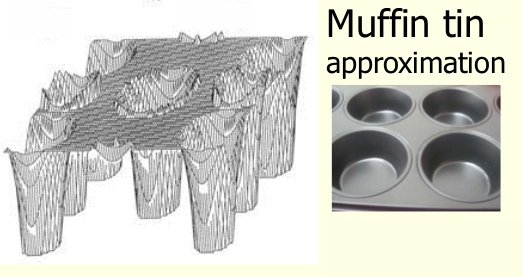
\includegraphics[height=1.10in,width=1.92in,viewport=1 22 507 295,clip]{Figures/Muffin-tin.png}}
\subfigure[\textrm{Division of the unit cell into spheres(I) and into interstitial region(II)}]{
\label{Semi-local-space}
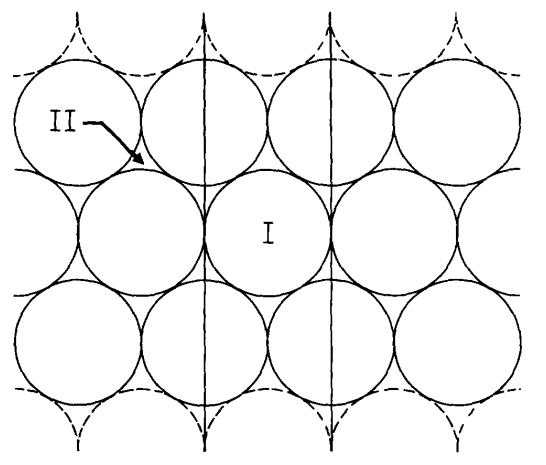
\includegraphics[height=1.45in,width=1.92in,viewport=1 20 515 435,clip]{Figures/Muffin-Tin.png}}
%\caption{\tiny \textrm{Division of the unit cell into spheres(I) and into interstitial region(II)}}%(与文献\cite{EPJB33-47_2003}图1对比)
\label{Muffin_tin-1}
\end{figure}
\textrm{Muffin-tin}近似是\textrm{Johnson}采用$\chi_{\alpha}$方法计算分子体系的交换-相关时,引入多重散射(\textrm{Multiple scattering})理论时提出的%,\textrm{Muffin-tin}直译为“松饼罐头”,意思是把分子中的原子看成堆在一起的圆球罐

\textcolor{red}{\textrm{MT}球近似与多重散射理论有密切的关联}
}

\frame
{
\frametitle{\textrm{APW}方法}
\begin{figure}[h!]
\centering
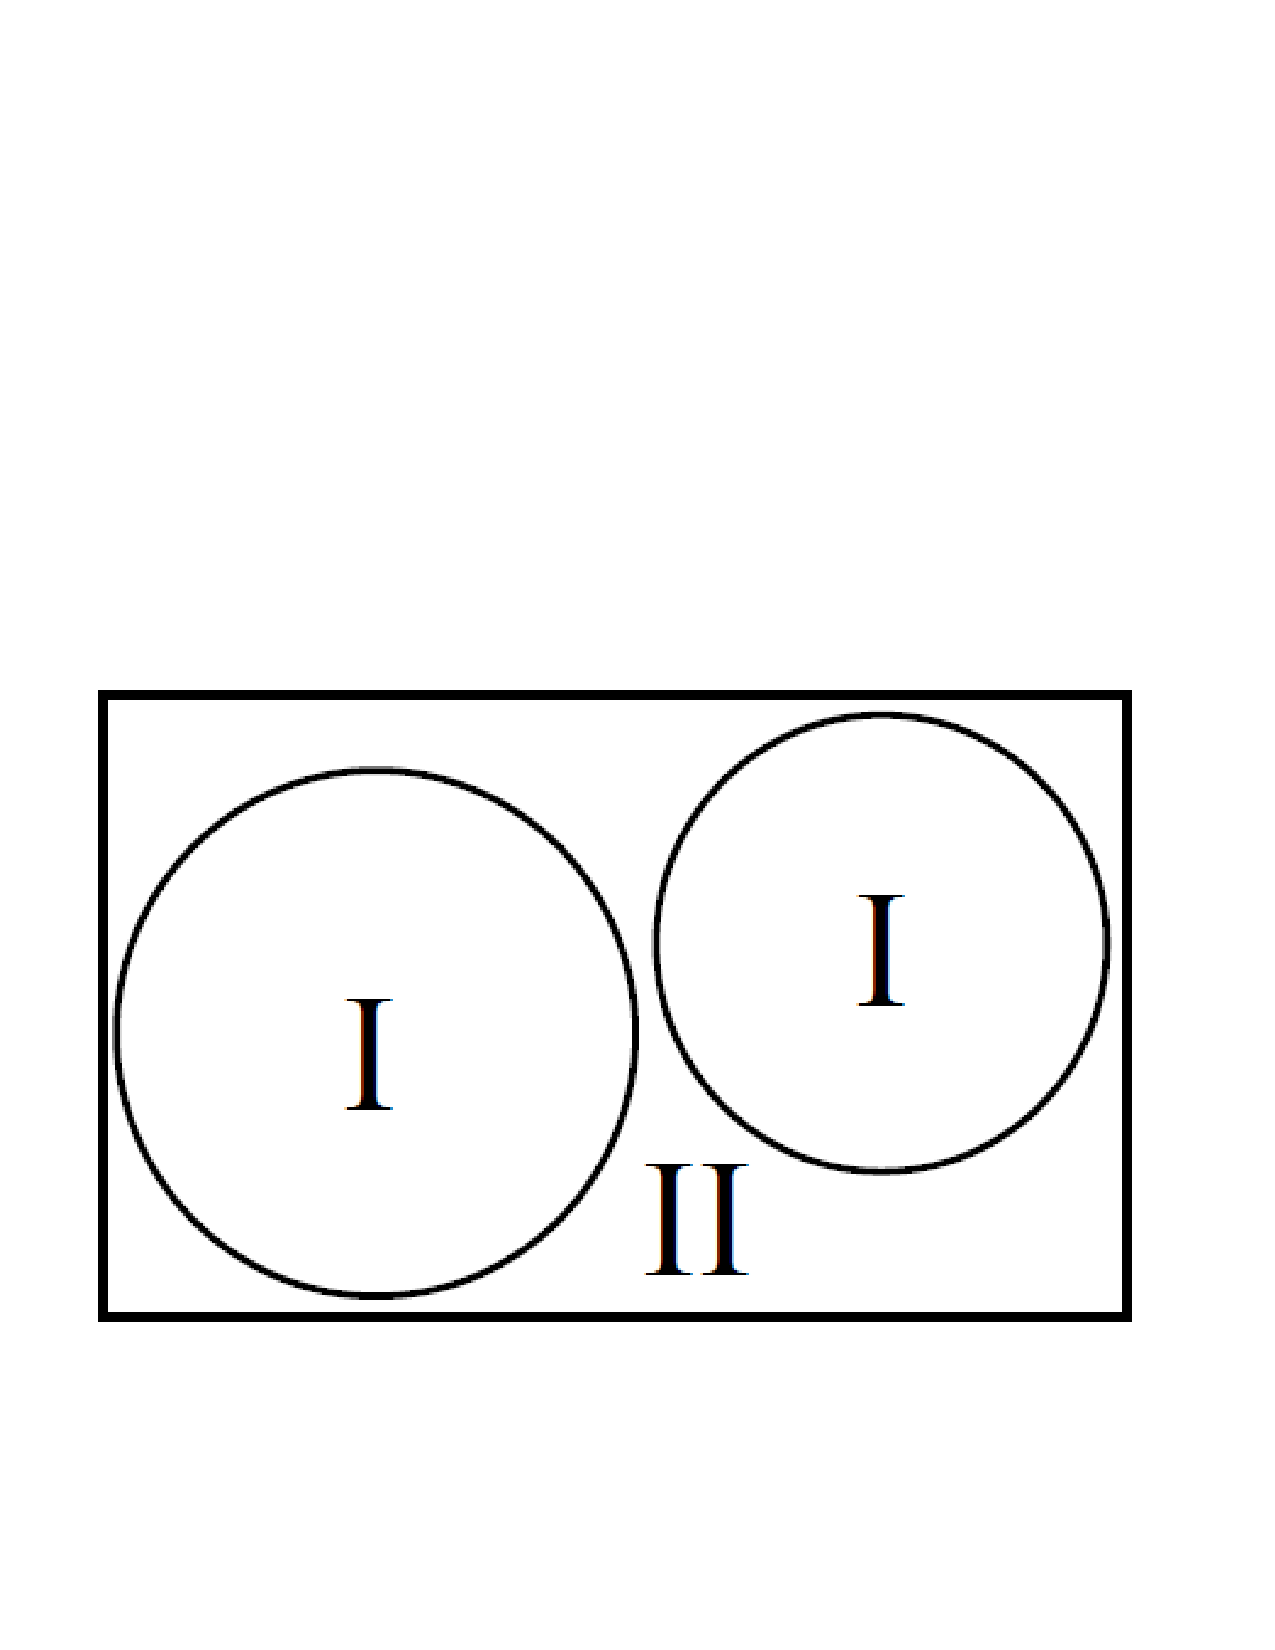
\includegraphics[height=1.10in,width=1.80in,viewport=40 150 545 465,clip]{Figures/Muffin_tin.pdf}
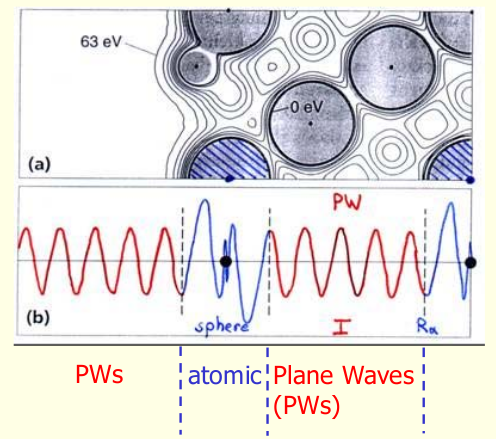
\includegraphics[height=1.10in,width=1.45in,viewport=1 20 485 435,clip]{Figures/APW.png}
\caption{\tiny \textrm{Partitioning of the unit cell into atomic spheres(I) and an interstitial region(II)}}%(与文献\cite{EPJB33-47_2003}图1对比)
\label{Muffin_tin-2}
\end{figure}
\begin{displaymath}
\hskip -28pt\footnotesize \varphi(\vec k_j,\vec r)=\left\{
  \begin{aligned}
    &\Omega^{-1/2}\exp[i\vec k_j\cdot\vec r],&|\vec r-\vec r_s|>R_{\mathrm{MT}}^s\\
    &\sum_{lm}A_{lm}u_l(|\vec r-\vec r_s|,E)Y_{lm}(\widehat{\vec r-\vec r_s}),&|\vec r-\vec r_s|\leqslant R_{\mathrm{MT}}^s
  \end{aligned}
\right.
\end{displaymath}
}

\frame
{
	\frametitle{空间两部分函数在球面上的衔接}
	\textrm{Huygens}原理:~\textcolor{blue}{平面波可以在各个原子球中心用球谐函数展开}:
	\begin{displaymath}
		\mathrm{e}^{\mathrm{i}\vec k\cdot\vec r}=4\pi\sum_{l=0}^{\infty}\sum_{m=-l}^l\mathrm{i}^lj_l(|\vec k|r)Y_{lm}^{\ast}(\hat{\vec k})Y_{lm}(\hat{\vec r})
	\end{displaymath}
	其中$j_l(|\vec k|r)$是$l$-阶球\textrm{Bessel}函数,$\hat{\vec k}$和$\hat{\vec r}$分别是矢量$\vec k$和$\vec r$与直角坐标$z$-轴的夹角$\theta$和$\varphi$

	要求空间中不同区域函数在球面上连续,可调参数$A_{lm}^{\vec k}$可为下式确定
\begin{displaymath}
	A_{lm}^{\vec k}=4\pi\mathrm{e}^{\mathrm{i}\vec k\cdot\vec r_s}\mathrm{i}^lY_{lm}^{\ast}(\hat{\vec k})j_l(|\vec k|R_{MT}^s)/u_l(R_{MT}^s,E)
\end{displaymath}
\textrm{APW}的问题:\textcolor{blue}{球面参数$A_{lm}^{\vec k}$对能量$E$依赖,由此构造的久期方程\footnote{\fontsize{7.2pt}{6.2pt}\selectfont{久期方程\textrm{secular~equation},\textrm{secular}来自拉丁语\textrm{saeculum},本意为一代人、一个时期、一个时代、一个世界等意思。其名词在拉丁语中就作为世纪讲。汉译\textrm{secular}为久期,是取\textrm{long-term}的意思(实为慢,\textrm{slow~in~comparison~to~the~annual~motion}的意思),与期待\textrm{(expectation)}无关\upcite{PhysCN40-477_2011}。}}非线性的}
}

\frame
{
\frametitle{\textrm{LAPW}方法}
%\small\textrm{APW}方法的困难,久期方程不能化成广义本征值方程的形式(久期方程对能量$E$是非线性的)为了克服这一困难,人们提出线性化方法,
\textrm{O.~K.~Andersen~}提出\textrm{LAPW}方法\upcite{Singh}:将$u_l(r,E)$在某一合适的$E_l$值附近对$E$的一阶微商{$\left.\dfrac{\textrm{d}u_l(r,E)}{\textrm{d}E}\right|_{E_l}\equiv\dot u_l(r,E_l)$}\\代入\textrm{APW}基函数中可得\textrm{LAPW}方法的基函数:
{\fontsize{7.5pt}{3.3pt}\selectfont
$$\hskip -14pt \varphi(\vec k_j,\vec r)=\left\{
  \begin{aligned}
    &\Omega^{-1/2}\exp[i\vec k_j\cdot\vec r],&|\vec r-\vec r_s|>R_{\mathrm{MT}}^s\\
    &\sum_{lm}[A^{\vec k_j}_{lm}u_l(|\vec r-\vec r_s|,E_l)+B^{\vec k_j}_{lm}\dot u_l(|\vec r-\vec r_s|,E_l)]Y_{lm}(\widehat{\vec r-\vec r_s}),&|\vec r-\vec r_s|\leqslant R_{\mathrm{MT}}^s
  \end{aligned}
\right.$$
%$$\Psi_{\vec k}(\vec r)=\int_{\Omega}\tilde G_{\vec k}(\vec r-\vec r\,^\prime;E)V(\vec r\,^\prime)\Psi_{\vec k}(\vec r\,^\prime)\textrm{d}\vec r\,^\prime$$
根据基函数在\textrm{MT}球面上连续到一阶,确定系数$A^{\vec k}_{lm}$,$B^{\vec k}_{lm}$的值。}
\begin{figure}[h!]
	\vskip -3pt
\centering
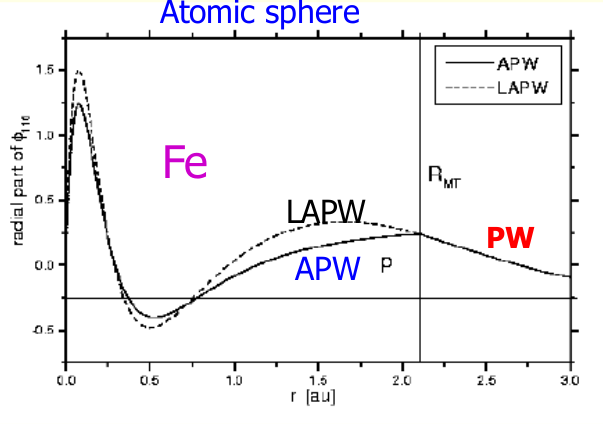
\includegraphics[height=1.10in,width=1.88in,viewport=1 20 585 435,clip]{Figures/WIEN2k-LAPW.png}
\caption{\tiny \textrm{Partitioning of the unit cell into atomic spheres(I) and an interstitial region(II)}}%(与文献\cite{EPJB33-47_2003}图1对比)
\label{Muffin_tin-3}
\end{figure}
}

\frame
{
	\frametitle{\textrm{Ghost~band}的表现}
	\fontsize{9.2pt}{4.2pt}\selectfont{只有价电子的波函数与芯电子波函数完全正交,能带计算中才能确保芯层与价层电子的完全分离。但实际计算时,该正交条件很难严格保证,因此一旦价电子波函数严重偏离正交条件,计算的能带中会在本不存在能带的区域出现电子结构分布(称为\textrm{Ghost~band}),这部分电子结构源自构造价电子波函数的能量参数$\varepsilon_l$与芯层电子能量差别太大,无法保持与芯层电荷严格正交引起的}
\begin{figure}[h!]
\centering
\vspace*{-0.10in}
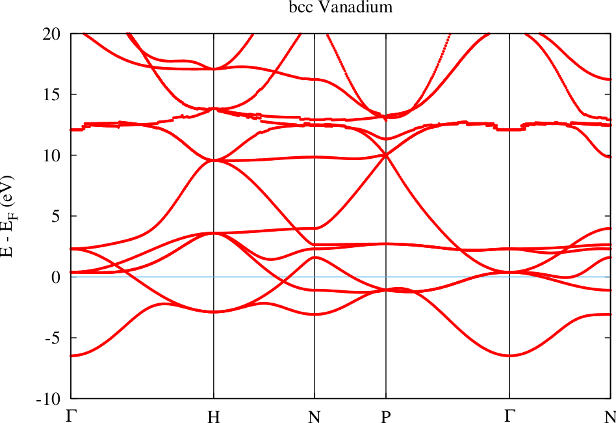
\includegraphics[height=1.50in,width=1.98in,viewport=0 0 450 320,clip]{Figures/Ghostband-Vanadium-1.png}
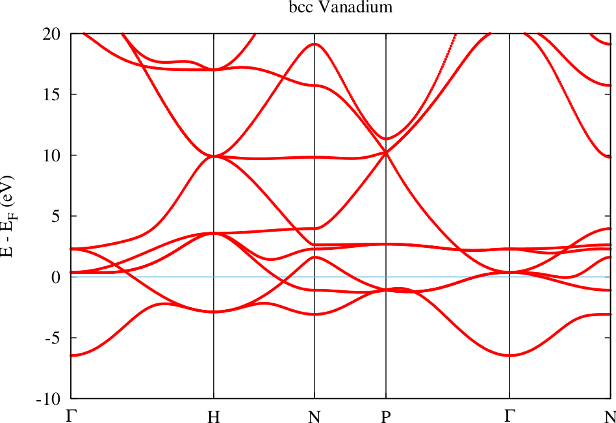
\includegraphics[height=1.50in,width=1.98in,viewport=0 0 450 320,clip]{Figures/Ghostband-Vanadium-4.png}
\caption{\fontsize{7.2pt}{4.2pt}\selectfont{\textrm{The band structure of bcc Vanadium. %In the calculation, all electrons up to the 3p states were treated as core electrons, all other electrons as valence electrons. 
\\Left:~Between 10 and 15 eV above the Fermi energy a strange band with nearly no dispersion can be observed. The vanishing dispersion of the band is a typical property of ghost bands.}}}%(与文献\cite{EPJB33-47_2003}图1对比)
\label{Ghost-band}
\end{figure}
}

\frame
{
	\frametitle{\textrm{semi-core}与\textrm{Ghost-band}}
\begin{figure}[h!]
\centering
\vspace*{-0.2in}
\hspace*{-0.2in}
\subfigure[\textrm{Windows with a semi-core state}]{
\label{Semi-local-1}
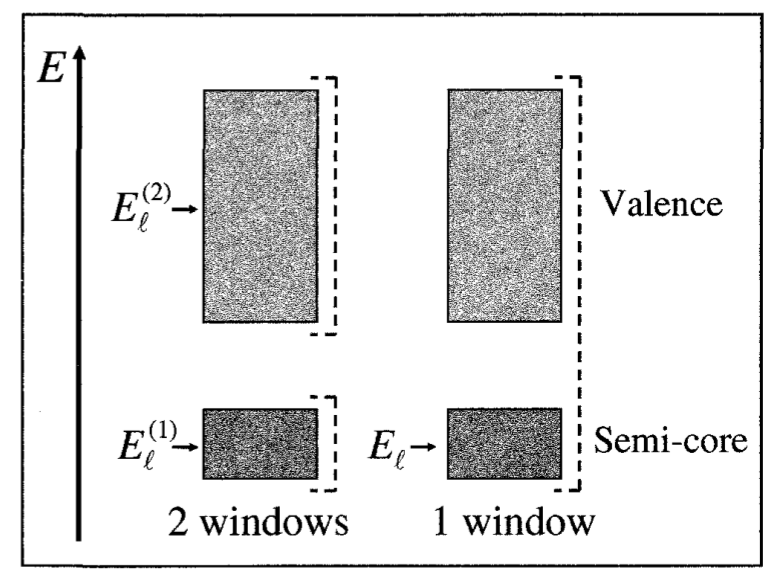
\includegraphics[height=1.88in,width=2.35in,viewport=0 0 785 615,clip]{Figures/Ghost-Multi_Windows.png}}
\subfigure[\textrm{Variation of a semi-core and a valence band with $E_l$}]{
\label{Semi-local-2}
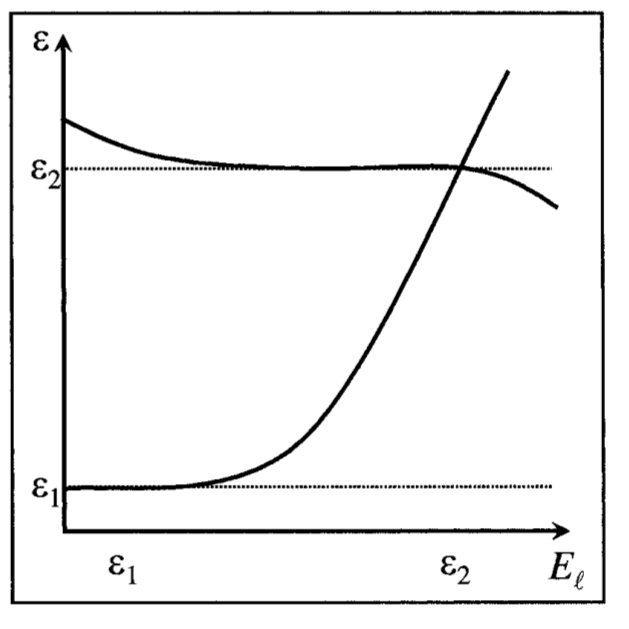
\includegraphics[height=1.88in,width=1.54in,viewport=0 0 625 650,clip]{Figures/Ghost-Multi_energy.png}}
\label{Semi-local}
\end{figure}
}

\frame
{
\frametitle{\textrm{LO}基函数}
为提高\textrm{LAPW}方法的变分自由度,在同一能量范围处理半芯态(接近价态的能量较高的芯态)和价态,可添加与$\vec k$无关的基函数,称为局域轨道(\textrm{local orbitals, LO})%。据此构造的基函数称为%包含两个指定能量的径向波函数和其中一个能量导数,这样的基函数即LAPW+
或\textrm{LO}基函数:
{
{\fontsize{8.5pt}{4.5pt}\selectfont
$$\hskip -10pt \phi_{lm}^{\mathrm{LO}}(\vec r)=\left\{
  \begin{aligned}
    &[A_{lm}u_l(r,E_{1,l})+B_{lm}\dot u_l(r,E_{1,l})+C_{lm}u_l(r,E_{2,l})]Y_{lm}(\hat{\vec r})\quad&r\leqslant R_{\mathrm{MT}}^s\\
    &0 &r>R_{\mathrm{MT}}^s
\end{aligned}
\right.$$}}

类似地,根据$\phi_{lm}^{\mathrm{LO}}(\vec r)$在\textrm{MT}球面上的数值为零、一阶导数为零,并且$\phi_{lm}^{\mathrm{LO}}(\vec r)$在\textrm{MT}球内归一化的要求,可以确定系数$A_{lm}$,$B_{lm}$,$C_{lm}$的值。
\begin{figure}[h!]
	\vspace{-15pt}
\centering
\hspace{15pt}
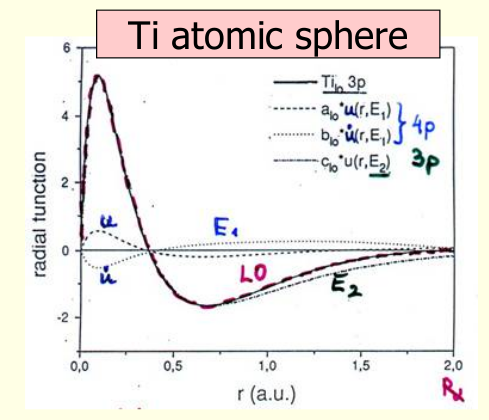
\includegraphics[height=1.45in,width=1.55in,viewport=50 10 470 415,clip]{Figures/WIEN2k-lo.png}
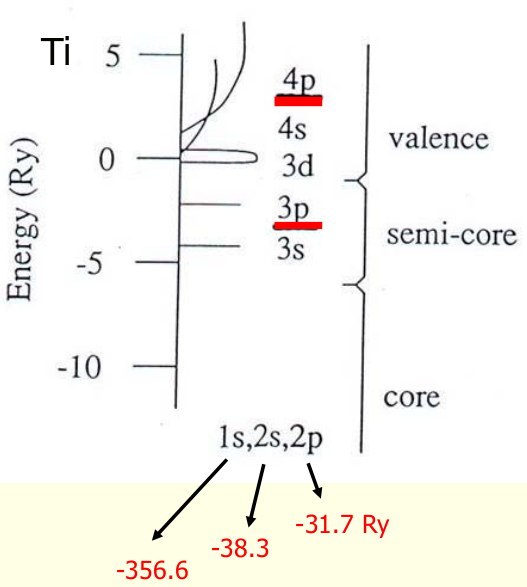
\includegraphics[height=1.45in,width=1.45in,viewport=5 1 570 570,clip]{Figures/semi-core.png}
\caption{\tiny \textrm{}}%(与文献\cite{EPJB33-47_2003}图1对比)
\label{Muffin_tin_LO}
\end{figure}
}

\frame
{
\frametitle{\textrm{APW+lo}基函数}
\textrm{Sj\"ostedt}等发现上述\textrm{LAPW}方法并非是\textrm{APW}方法线性化的最有效方法。采用指定能量参数$E_l$的\textrm{APW}形式的径向波函数,外加\textrm{APW}型局域轨道(\textrm{local orbit, lo})基函数,是更有效的方案,称为\textrm{APW+lo}方法\upcite{SSC114-15_2000}。
$$  \varphi(\vec k_j,\vec r)=\left\{
  \begin{aligned}
    &\sum_{lm}[A^{\vec k_j}_{lm}u_l(r,E_l)]Y_{lm}(\hat{\vec r})\quad&r\leqslant R_{\mathrm{MT}}^s\\
    &\Omega^{-1/2}\exp(i\vec k_j\cdot\vec r) &r>R_{\mathrm{MT}}^s
  \end{aligned}\right.
  \label{eq:APW-basis}
$$
$$  \phi_{lm}^{\mathrm{lo}}(\vec r)=\left\{
  \begin{aligned}
  &[A_{lm}u_l(r,E_{1,l})+B_{lm}\dot u_l(r,E_{1,l})]Y_{lm}(\hat{\vec r})\quad&r\leqslant R_{\mathrm{MT}}^s\\
  &0&r>R_{\mathrm{MT}}^s
  \end{aligned}
\right.$$
\textrm{APW+lo}基函数式形式上与标准\textrm{LAPW}基函数式形式非常相似,但\textrm{APW+lo}基函数是平滑且一阶可微的,在\textrm{MT}球面上有动能对\textrm{Hamiltonian}的贡献需要计算。计算表明,采用\textrm{APW+lo}基组比标准\textrm{LAPW}基组计算效率高。
}

\subsection{全势的基本思想}
\frame
{
\frametitle{全势的基本思想}
全势\textrm{(Full Potential, FP)}是相对于赝势的概念,即\textcolor{blue}{电子运动过程中感受到其它粒子作用的真实效果}。
实际计算中,构造\textrm{LAPW}基组的\textrm{MT}势换成晶体势函数。一般地,在每个\textrm{MT}球内,势函数用球谐函数(或者是满足晶体对称性)展开,\textrm{MT}球外的势函数用\textrm{Fourier}级数展开:%\upcite{PRB13-5362_1976}
{\footnotesize$$ V(\vec r)=\left\{
  \begin{aligned}
    &\sum_{a,L}V_L^a(r)Y_L(\hat{\vec r})\quad &r\leqslant R_{\mathrm{MT}}^a\\
    &\sum_{\vec G_n}V_I(\vec G_n)\textrm{e}^{i\vec G_n\cdot\vec r} &\vec r\in\mathrm{II}
  \end{aligned}\right.
  \label{eq:solid-63}
$$}
这里$L$\,$\equiv$\,$l,m$,$\vec G_n$为倒格矢,$Y_L(\hat{\vec r})$是球谐函数,\textrm{II}为原子间隙
\begin{itemize}
	\item 在\textrm{MT}球内靠近原子核,势能具有原子型势能特征
	\item 在\textrm{MT}球外,要满足\textrm{Bloch}函数边界条件特征。
	\item 在\textrm{MT}球内外的势能表象不同,同样要求势能在\textrm{MT}球表面连续。
\end{itemize}
}

\frame
{
\frametitle{全势的基本思想}
\vspace*{-13pt}
\begin{figure}[h!]
\centering
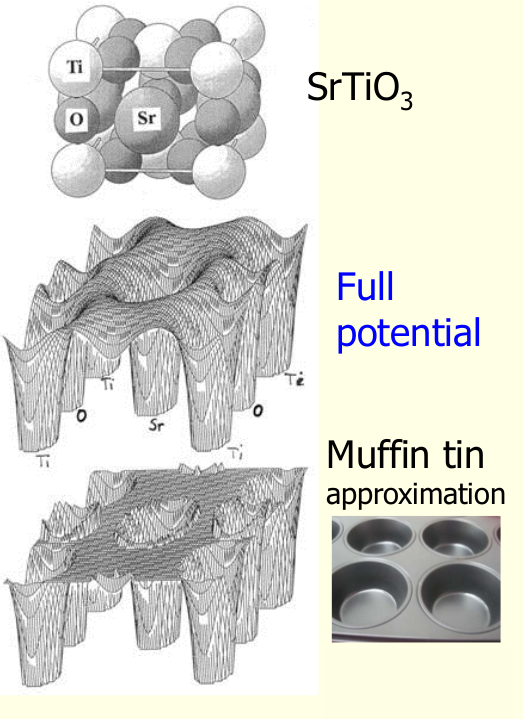
\includegraphics[height=2.70in,width=2.02in,viewport=1 22 507 715,clip]{Figures/MT_FP.png}
\caption{\tiny \textrm{From Muffin-tin Potential to Full Potential}}%(与文献\cite{EPJB33-47_2003}图1对比)
\label{Muffin_tin_FP}
\end{figure}
}

\frame
{
\frametitle{全势的基本思想}
由此得到晶体的势函数为\upcite{Nemoshkalenko-Antonov}
$$ V(\vec r)=V_{MT}(\vec r)+V_{WMT}(\vec r)+V_{NS}(\vec r)
  \label{eq:solid-64}
$$
\begin{itemize}
	\item $V_{MT}(\vec r)$是简单的\textrm{MT}势(包括\textrm{MT}球内球对称部分和\textrm{MT}球外常数势)
	\item $V_{WMT}(\vec r)$表示\textrm{MT}球外势能\textrm{Fourier}展开对\textrm{MT}常数势的偏离,仅在\textrm{MT}球外非零,球内为零
	\item $V_{NS}(\vec r)$是势能在\textrm{MT}球内对球对称性的偏离,只在\textrm{MT}球内有非零值
\end{itemize}
\textbf{\large 为求得交换-相关势$V_{\mathrm{XC}}$,将电荷密度也采用类似的形式展开。}
}

\frame
{
\frametitle{全势方法在$\vec k$空间中的实现}
根据电动力学定理:\\\textcolor{blue}{如果球\textrm{S}内的电荷密度分布$\rho(\vec r)$,在球外某点$\vec r$产生的势是由电荷密度的多极矩确定}:
\begin{figure}[h!]
\vspace*{-15pt}
\centering
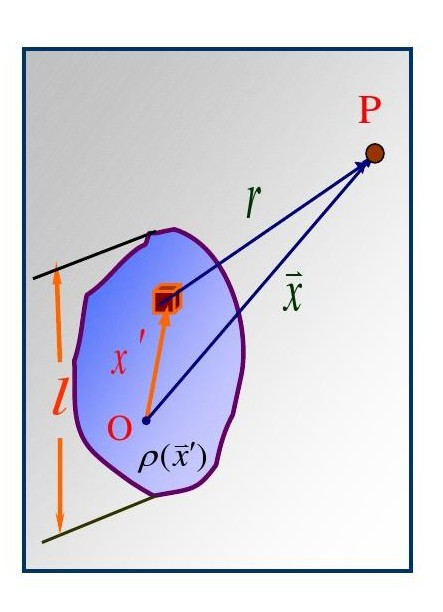
\includegraphics[height=1.25in,width=1.32in,viewport=1 22 507 575,clip]{Figures/potential_multipole.jpg}
%\caption{\tiny \textrm{From Muffin-tin Potential to Full Potential}}%(与文献\cite{EPJB33-47_2003}图1对比)
\label{Potential-multipole}
\end{figure}
\begin{displaymath}
	V(\vec r)=\sum_{l=0}^{\infty}\sum_{m=-l}^{l}\dfrac{4\pi}{2l+1}q_{lm}\dfrac{Y_{lm}(\hat{\vec r})}{r^{l+1}}
\end{displaymath}
其中多极矩$q_{lm}$由下式计算
\begin{displaymath}
	q_{lm}=\int_SY_{lm}^{\ast}(\hat{\vec r})r^l\rho(\vec r)\mathrm{d}^3r
\end{displaymath}
}

\frame
{
	\frametitle{全势方法在$\vec k$空间的实现}
\textrm{Weiner}提出全势计算的实现方法\upcite{JMP22-2433_1981}:~\\
\begin{itemize}
	\item 将\textrm{MT}球外的电荷密度$\rho_I(\vec r)$扩展到球内
	\begin{displaymath}
		\rho_I(\vec r)=\sum_{\vec K}\rho_I(\vec K)\mathrm{e}^{\mathrm{i}\vec K\cdot\vec r_s}\mathrm{e}^{\mathrm{i}\vec K\cdot(\vec r-\vec r_s)}
	\end{displaymath}
	这部分电荷在每个球内的多极矩展开$q_{lm}^{s,PW}$
	\begin{displaymath}
		\begin{aligned}
			q_{lm}^{s,PW}=&\dfrac{\sqrt{4\pi}}3{R_{MT}^s}^3\rho_I^{(\vec K=0)}\delta_{l0}+\sum_{\vec K\neq0}4\pi\mathrm{i}^l\rho_I(\vec K){R_{MT}^s}^{l+3}\\
			&\times\dfrac{j_{l+1}(|\vec K|R_{MT}^s)}{\vec K\cdot\vec R_{MT}^s}\mathrm{e}^{\mathrm{i}\vec K\cdot\vec r_s}Y_{lm}^{\ast}(\hat{\vec K})
		\end{aligned}
	\end{displaymath}
\end{itemize}
}

\frame
{
	\frametitle{全势方法在$\vec k$空间的实现}
\begin{itemize}
	\item 根据\textrm{MT}球内的电荷密度分布,电子密度$\rho_s(\vec r)$在正空间分布的多极矩$q_{lm}^{s,MT}$
\begin{displaymath}
	q_{lm}^{s,MT}=\int_0^{R_{MT}^s}Y_{lm}^{\ast}(\hat{\vec r})r^l\rho_s(\vec r)\mathrm{d}^3r
\end{displaymath}
由此得到在\textrm{MT}球内,真实电荷密度多极展开多极矩与延伸到球内的平面波电荷多极矩之差
	\begin{displaymath}
		\delta q_{lm}^{s,MT}=q_{lm}^{s,MT}-q_{lm}^{s,PW}
	\end{displaymath}
\end{itemize}
}

\frame
{
	\frametitle{全势方法在$\vec k$空间的实现}
\begin{itemize}
	\item 构造赝电荷密度$\tilde\rho(\vec r)$,要求$\tilde\rho(\vec r)$在空间分布平缓,其多级矩$\tilde q_{lm}^{s,MT}$即为$\delta q_{MT}^s$,由此得到赝电荷密度的\textrm{Flourier}变换为
	\begin{displaymath}
		\begin{aligned}
			\tilde\rho_s(\vec K)=&\dfrac{4\pi}{\Omega}\sum_{lm,s}(-\mathrm{i})^l\left\{\dfrac{(-1)^n\tilde q_{lm}^{s,MT}}{2^nn!a_n{R_{MT}^s}^{2l+2n+3}}\dfrac{(2l+2n+3)!!}{(2l+1)!!}\right\}\\
			&\times\left\{(-1)^n2^nn!a_n{R_{MT}^s}^{l+2n+3}\dfrac{j_{l+n+1}(|\vec K|R_{MT}^s)}{(\vec K\cdot\vec R_{MT}^s)^{n+1}}\right\}\\
			&\times\mathrm{e}^{\mathrm{-i}\vec K\cdot\vec r_s}Y_{lm}^{\ast}(\hat{\vec K})
		\end{aligned}
	\end{displaymath}
\end{itemize}
}

\frame
{
	\frametitle{全势方法在$\vec k$空间的实现}
\begin{itemize}
	\item 在$\vec k$空间内,用平面波电荷密度$\rho_I(\vec K)$叠加\textrm{MT}球内赝电荷密度$\tilde\rho_s(\vec K)$:
		\begin{displaymath}
			\tilde\rho(\vec K)=\tilde\rho_s(\vec K)+\rho_I(\vec K)
		\end{displaymath}
		\textcolor{blue}{这样构造的赝电荷密度,在\textrm{MT}球外产生的势与真实电荷密度分布产生的势相等}:~根据\textrm{Coulomb}定理计算得到\textrm{Coulomb}势在间隙区的表达式$V_I(\vec K)$(\textrm{Poisson}方程)
		\begin{displaymath}
			V_I(\vec K)=\dfrac{4\pi\tilde\rho(\vec K)}{|\vec K|^2}
		\end{displaymath}
\end{itemize}
}

\frame
{
	\frametitle{全势方法在$\vec k$空间的实现}
\begin{itemize}
	\item 在\textrm{MT}球面内,根据真实的电荷密度分布$\rho_s(\vec r)$和球面上的电势值(球形\textrm{Dirichlet}边值条件),计算\textrm{MT}球内电子的\textrm{Coulomb}势$V_s(\vec r)$
		\begin{displaymath}
			\begin{aligned}
				V_s(\vec r)=&\sum_{lm}Y_{lm}(\hat{\vec r})\left[\dfrac{4\pi}{2l+1}\bigg\{\dfrac1{r^l+1}\int_0^r\mathrm{d}r^{\prime}{r^{\prime}}^{l+2}\rho_{lm}(\vec r^{\prime})\right.\\
					&+r^l\int_r^{R_{MT}^s}\mathrm{d}r^{\prime}(r^{\prime})^{1-l}\rho_{lm}(\vec r^{\prime})\bigg\}\\
					&+\bigg(\dfrac r{R_{MT}^s}\bigg)^l4\pi\mathrm{i}^l\\
					&\times\sum_{K\neq0}\left.\dfrac{4\pi}{|\vec K|^2}\tilde\rho_I(\vec K)Y_{lm}^{\ast}(\vec K)\dfrac{\vec K\cdot\vec R_{MT}^sj_{l-1}(|\vec K|R_{MT}^s)}{2l+1}\right]
			\end{aligned}
		\end{displaymath}
\end{itemize}
}

\subsection{全势方法下的总能量计算}
\frame
{
	\frametitle{总能量的计算}
	\textrm{Weinert}等利用核\textrm{Coulomb}势的发散项与电子动能-势能项发散项解析抵消属性,提出新的总能量计算方法\upcite{PRB26-4571_1982}:
	根据\textrm{DFT},体系总能量分解为
	\begin{displaymath}
		E[\rho]=T_s[\rho]+U[\rho]+E_{\mathrm{XC}}[\rho]
	\end{displaymath}
	其中$U[\rho]$包含全部(经典)电荷相互作用:~
	\begin{displaymath}
		U[\rho]=\dfrac12\left[\int\dfrac{\rho(\vec r)\rho(\vec r^{\prime})}{|\vec r-\vec r^{\prime}|}\mathrm{d}\vec r\mathrm{d}\vec r^{\prime}-2\sum_{\alpha}Z_{\alpha}\int\dfrac{\rho(\vec r)\mathrm{d}\vec r}{|\vec r-\vec R_{\alpha}|}+\sum_{\alpha,\beta}{}^{\prime}\dfrac{Z_{\alpha}Z_{\beta}}{|\vec R_{\alpha}-\vec R_{\beta}|}\right]
	\end{displaymath}
	这里$Z_{\alpha}$是位于$R_{\alpha}$的核电荷
}

\frame
{
	\frametitle{\textrm{Madelung}常数与\textrm{Madelung}势}
\begin{figure}[h!]
\vspace*{-10pt}
\centering
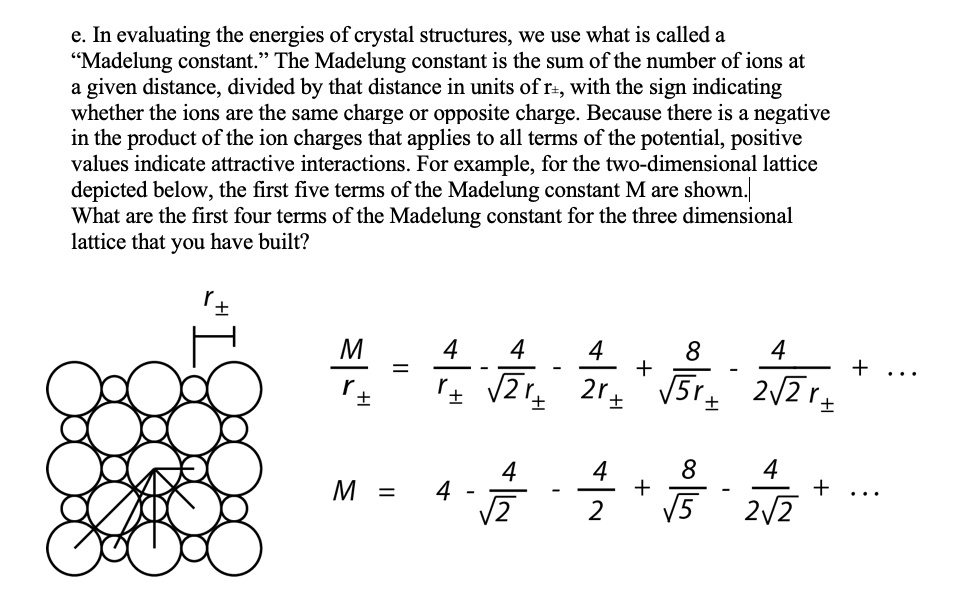
\includegraphics[height=0.75in,width=2.50in,viewport=0 15 950 330,clip]{Figures/Madelung_Constant.jpg}\\
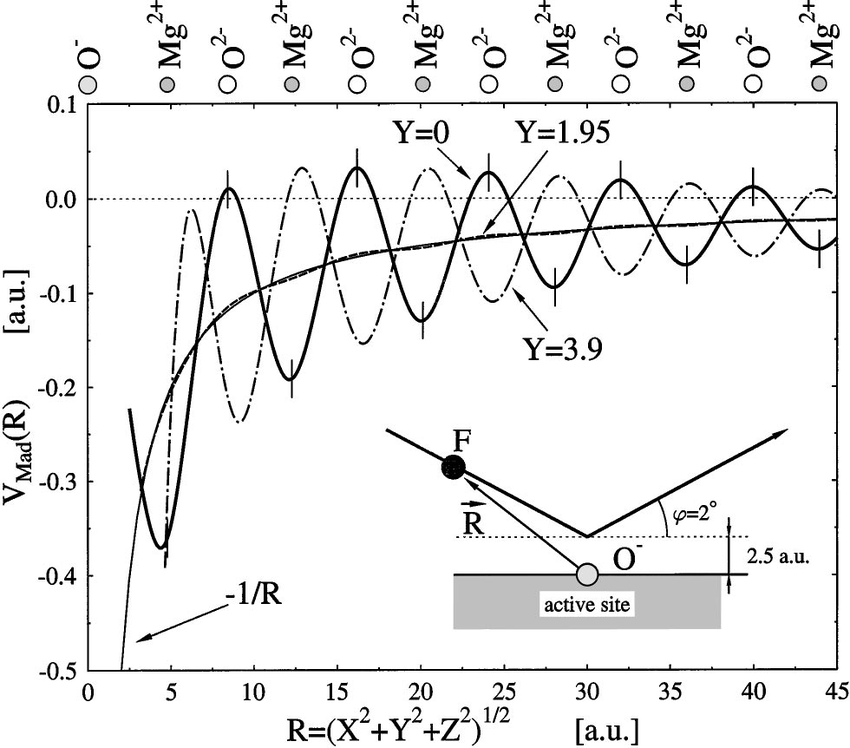
\includegraphics[height=2.15in,width=2.50in,viewport=0 0 850 750,clip]{Figures/Madelung-potential-V-Mad-for-different-impact-parameters-Y-along-a-grazing-trajectory.png}
%\caption{\tiny \textrm{From Muffin-tin Potential to Full Potential}}%(与文献\cite{EPJB33-47_2003}图1对比)
\label{Madelung-Constant_Potential}
\end{figure}
}

\frame
{
	\frametitle{总能量的计算}
	记经典\textrm{Coulomb}势
	\begin{displaymath}
		V_c(\vec r)=\int\dfrac{\rho(\vec r^{\prime})}{|\vec r-\vec r^{\prime}|}\mathrm{d}\vec r^{\prime}-\sum_{\alpha}\dfrac{Z_{\alpha}}{|\vec r-\vec R_{\alpha}|}
	\end{displaymath}
	定义\underline{\textcolor{red}{广义的\textrm{Madelung}势}}
	\begin{displaymath}
		V_M(\gamma_{\nu})=\int\dfrac{\rho(\vec r)\mathrm{d}\vec r}{|\vec r-\vec \gamma_{\nu}|}-\sum_{\alpha}{}^{\prime}\dfrac{Z_{\alpha}}{|R_{\alpha}-\gamma_{\nu}|}
	\end{displaymath}
	\textcolor{red}{注意}:~\textcolor{blue}{位于\textrm{$\gamma_{\nu}$的\textrm{Madelung}势是晶体中除该点核电荷$Z_{\nu}$之外,所有其他电荷在该点产生电势之和}}

	如果体积为$\Omega$的晶体包含$N$个原胞,则$U$表示为
	\begin{displaymath}
		U=\dfrac N2\left[\int_{\Omega}\rho(\vec r)V_c(\vec r)\mathrm{d}\vec r-\sum_{\nu}Z_{\nu}V_M(\vec \gamma_{\nu})\right]
	\end{displaymath}
	其中对$\nu$的求和遍历原胞中所有的核位置$\gamma_{\nu}$
}

\frame
{
	\frametitle{总能量的计算}
	假设已知晶体中全部电荷产生\textrm{Coulomb}势,并设原点$\gamma_{\nu}$半径为$R_{\nu}$的球面上的球平均势是$S_0(R_{\nu})$,则除了球面上除核电荷$Z_{\nu}$外的平均势为
	\begin{displaymath}
		S(R_{\nu})=S_0(R_{\nu})+Z_{\nu}/R_{\nu}
	\end{displaymath}
	根据球形\textrm{Dirichlet}边值条件,$\gamma_{\nu}$处的\textrm{Coulomb}势,可由球内电荷密度分布$\rho(\vec r)$和$S(R_{\nu})$确定。

	球内的电荷密度用球谐函数展开
	\begin{displaymath}
		\rho(\vec r_{\nu})=\sum_{lm}\rho_{lm(r_{\nu})}Y_{lm}(\hat{\vec r}_{\nu})
	\end{displaymath}
	并记球内电子电荷为$Q_{\nu}$,由此可得
	\begin{displaymath}
		\begin{aligned}
			V_M(\gamma_{\nu})=&\dfrac1{R_{\nu}}\big[R_{\nu}S_0(R_{\nu})+Z_{\nu}-Q_{\nu}\big]+\sqrt{4\pi}\int_0^{R_{\nu}}\mathrm{d}rr\rho_{00}(r_{\nu})\\
			=&\dfrac1{R_{\nu}}\big[R_{\nu}S_0(R_{\nu})+Z_{\nu}-Q_{\nu}\big]+\left\langle\dfrac1r\rho(\vec r)\right\rangle_{\nu}
		\end{aligned}
	\end{displaymath}
}

\frame
{
\frametitle{总能量的计算}
原胞内的电子动能为
\begin{displaymath}
	\hspace*{-10pt}
	T_s[\rho]=\sum_i\varepsilon_i-\int_{\Omega}V_{e\!f\!f}(\vec r)\mathrm{d}\vec r=\sum_i\varepsilon_i-\int_{\Omega}V_c(\vec r)\rho(\vec r)\mathrm{d}\vec r-\int_{\Omega}\mu_{\mathrm{XC}}(\vec r)\rho(\vec r)\mathrm{d}\vec r
\end{displaymath}
由此可得\textrm{WS}原胞内的总能量的表达式
{\fontsize{9.5pt}{5.2pt}\selectfont
\begin{displaymath}
\begin{split}
	E_T=&\sum_i\varepsilon_i-\frac12\int_{\Omega}\underline{\textcolor{blue}{\rho(\vec r)}}[\underline{\textcolor{blue}{V_c(\vec r)}}+2\mu_{XC}(\vec r)]\mathrm{d}\vec r-\frac12\sum_{\nu}\underline{\textcolor{blue}{Z_{\nu}V_M(\vec r_{\nu})}}+E_{\mathrm{XC}}[\rho] \\
	=&\sum_i\varepsilon_i-\frac12\left(\underline{\textcolor{blue}{\int_{\Omega}\rho(\vec r)V_c(\vec r)\mathrm{d}\vec r}}+\underline{\textcolor{blue}{\sum_{\nu}Z_{\nu}\bigg\langle\frac1r\rho(\vec r)\bigg\rangle_{\nu}}}\right)-%\dfrac12
   \int_{\Omega}\rho(\vec r)\mu_{\mathrm{XC}}(\vec r)\mathrm{d}\vec r \\
   &-\frac12\underline{\textcolor{blue}{\sum_{\nu}\frac{Z_{\nu}}{R_{\nu}}[R_{\nu}S_0(R_{\nu})+Z_{\nu}-Q_{\nu}]}}+E_{\mathrm{XC}}[\rho]
\end{split}
\end{displaymath}
}
这里$V_c(\vec r)\!=\!\displaystyle\int\dfrac{\rho(\vec r\,^\prime)}{|\vec r-{\vec r}\,^\prime|}\mathrm{d}\vec r\,^\prime-\sum\limits_{\alpha}\dfrac{Z_{\alpha}}{|\vec r-\vec r_{\alpha}|}$,$\mu_{\mathrm{XC}}$为交换-相关势。
}

\frame
{
\frametitle{原子核位置能量奇点排除}
核吸引势和\textrm{Coulomb}势在原子核位置都存在奇点,单独求和,总能量是发散的。

为排除奇点,将\textrm{Coulomb}势能和电荷密度在各原子核附近用球谐函数展开,在原子核附近,有
{\fontsize{9.0pt}{5.2pt}\selectfont
\begin{displaymath}
  \begin{split}
    &\int_{\Omega}\rho(\vec r)V_c(\vec r)\mathrm{d}\vec r+Z_{\nu}\sqrt{4\pi}\int_0^{R_{\nu}}\mathrm{d}rr^2\frac{\rho_{00}(r)}r\\
    =&\sqrt{4\pi}\int_0^{R_{\nu}}\mathrm{d}rr^2\rho_{00}(\vec r)\left(\textcolor{red}{\dfrac1{\sqrt{4\pi}}V_{00}(r)}+\textcolor{red}{\frac{Z_{\nu}}r}\right)+\sum_{lm>0}\int_0^{R_{nu}}\mathrm{d}rr^2\rho_{lm}(r)V_{lm}(r)
  \end{split}
\end{displaymath}
}
\textcolor{blue}{\textrm{Coulomb}势的奇点只出现在$V_{00}(r)$中,将$V_{00}(r)$写成核的点电荷势与源于电子的平缓的势$\hat V_{00}(r)$两部分之和}:~
\textcolor{red}{$$V_{00}(r)=-\sqrt{4\pi}\frac{Z_{\nu}}r+\textcolor{red}{\hat V_{00}(r)}$$}
可以看出\textrm{Coulomb}势的奇点被消去了。\\有必要指出的是,这样方式可以将总能量中的奇点排除,但是\textcolor{red}{单独每一项在原子核位置仍然是发散的}。
}

\frame
{
	\frametitle{\textrm{LDA~}近似下的总能量表达式}
\begin{itemize}
	\item 间隙区的电荷密度用平面波展开:{$\rho(\vec r)=\sum\limits_{\vec G}\rho(\vec G)\mathrm{e}^{i\vec G\cdot\vec r}$}
	\item 在\textrm{MT}球内,电荷密度用球谐函数展开,在动量空间中的展开形式为:{$\bar\rho_{lm}(r_{\nu})=4\pi i^l\sum\limits_{\vec G}\rho(\vec G)\mathrm{e}^{i\vec G\cdot\vec r_{\nu}}j_l(\vec G\cdot\vec r_{\nu})Y_{lm}^{\ast}(\vec G)$}
\end{itemize}
\textrm{LDA}近似下,{\fontsize{7.5pt}{4.2pt}\selectfont$$E_{\mathrm{XC}}[\rho]\approx\int_{\Omega}\rho(\vec r)\varepsilon_{\mathrm{XC}}(\vec r)\textrm{d}\vec r$$}
因此\textrm{WS}原胞内的晶体总能量可以写成:
{\fontsize{7.5pt}{4.2pt}\selectfont
\begin{displaymath}
  \begin{split}
\hskip -10pt	  E=&\sum_i\varepsilon_i-\Omega\sum_{\vec G}\rho(\vec G)\tilde V^{\ast}(\vec G)-\frac12\sum_{\nu}\dfrac{Z_{\nu}}{R_{\nu}}[Z_{\nu}-Q_{\nu}+R_{\nu}S_0(R_{\nu})]\\
    &-\sum_{\nu}\sum_{lm}\int_0^{R_{\nu}}\mathrm{d}rr^2\left[\rho_{lm}(r_{\nu})\left(\tilde V_{lm}^{\ast}(r_{\nu})+\dfrac{\sqrt{4\pi}}{2r_{\nu}}Z_{\nu}\delta_{l0}\right)-\bar\rho_{lm}(\vec r_{\nu})\bar V_{lm}^{\ast}(\vec r_{\nu})\right]
  \end{split}
  \label{eq:solid-83}
\end{displaymath}}
这里$\tilde V(\vec r)$和$\bar V_{lm}(\vec r)$根据都按下式计算:
{\fontsize{7.5pt}{4.2pt}\selectfont$$\tilde V(\vec r)=\frac12V_c(\vec r)-\varepsilon_{\mathrm{XC}}(\vec r)+\mu_{\mathrm{XC}}(\vec r)$$}
}

%-----------------------------------------------------------------------------------------------------------------------------------------------------------------------%
		\frame[allowframebreaks]
{
\begin{thebibliography}{99}
\frametitle{主要参考文献}
{\tiny
	\bibitem{PhysCN40-477_2011}曹则贤, \textit{Secular,equation}, \textit{物理}, \textbf{40} \textrm{(2011), 477}
	\bibitem{Singh}\textrm{D. J. Singh. \textit{Plane Wave, PseudoPotential and the LAPW method} (Kluwer Academic, Boston,USA, 1994)}
	\bibitem{Nemoshkalenko-Antonov}\textrm{V. V. Nemoshkalenko and V. N. Antonov. \textit{Computational Methods in Solid State Physics} (Gordon and Breach Science Publisher, Amsterdam, The Netherlands, 1998)}
	\bibitem{WIEN2k_UG}\textrm{P. Blaha, K. Schwarz, G. Madsen, D. Kvasnicka and J. Luitz. \textit{User's Guide of WIEN2K, An Augmented Plane Wave Plus Local Orbitals Program for Calculating Crystal Properties}. Vienna University of Technology, Inst. of Physical and Theoretical Chemistry, Vienna, Austria (2012)}
	\bibitem{PRB12-3060_1975}\textrm{O. K. Andersen. \textit{Phys. Rev.} B, \textbf{12} (1971), 3060}
	\bibitem{JMP22-2433_1981}\textrm{M. Weiner. \textit{J. Math. Phys.}, \textbf{22} (1981), 2433}
	\bibitem{PRB26-4571_1982}\textrm{M. Weinert, E. Wimmer and A. J. Freeman. \textit{Phys. Rev.} B, \textbf{26} (1982), 4571}
	\bibitem{SSC114-15_2000}\textrm{E. Sj\"ostedt, L. Nordstr\"om and D. J. Singh. \textit{Solid State Commun.}, \textbf{114} (2000), 15}
	\bibitem{Andersen_Book}\textrm{O. K. Andersen. \textit{Computational Methods in Band Theory} (Plenum, New York, USA, 1971)}
}
\end{thebibliography}
\nocite*{}
}
